\subsection{Resource tradeoffs and stronger native opportunity controls}
The current problem is joint routing quality: timing, planar wirelength, actual vertical occupation, legality, and complete execution cost. A legal candidate is not discarded solely because its CPD fails to beat strong A0. Final observed-state archive retention is separate from the transition policy. Strict timing and fixed timing/resource envelopes remain independent modes. Native FULL legality, physical delay, complete STA, hold guards, and rollback are mandatory. Intermediate resource-release and joint repairs may be tested in private transaction copies; only the complete combination commits. Occupancy on the fixed architecture is not a measured silicon-area or power reduction.

The automatic strict trajectory from pristine R1 accepts two own-current-STA moves and reaches13.228145689936355 ns, wire2068880/SB86/CB5072:1.441443\% lower CPD and twenty-eight fewer wire units, with unchanged vertical occupation. The second step expands the current critical-owner closure. It regresses one setup component that remains6.650274 ns above the new worst slack. The imported-state workflow takes960.935 s, excludes original routing and reused historical creation, and is not a cold algorithm runtime. This confirms a useful native selection/scope/schedule intervention on this case, not a new connection-search primitive or suite-wide improvement.

A separate six-arm paired resource experiment chooses the first currently ranked slack-bearing crossing-sharing branch. Both arms use the same native weighted objective, selected sinks, retained branches, device graph, and replacement opportunity. Only the optional allowed-crossing-source set changes. It limits the ON candidate to crossing sources already retained after pruning; the native transaction recomputes that set before each connection, updates real occupancy, and restores on exit. This restriction is a local ablation, not a permanent boundary on future joint search. Complete replacement and fresh native FULL/STA validate every candidate.

\begin{table}[t]
\centering\scriptsize
\caption{Completed crossing-domain pairs. ON minus OFF is a real resource tradeoff; all six final routes are legal.}
\begin{tabular}{lrrrrr}
\hline
Start & CPD(ns) & $\Delta$wire & $\Delta$SB & $\Delta$CB & ON core(s)\\
\hline
A0 &13.607436&92&0&$-1$&2.965\\
R1 &13.421610&96&0&$-1$&2.965\\
Tf &13.421610&96&0&$-1$&3.080\\
\hline
\end{tabular}
\end{table}
For every ON arm the exact CPD is unchanged, but some noncritical setup components regress. Strict-CPD and endpoint-vector modes reject these states. The preregistered shared envelope accepts them as a reduction in actual CB occupation: CPD at most13.607436066820355 ns, wire at most2076392, SB at most105, CB at most5072, with SB/CB nonincrease and one strict reduction. The unrestricted OFF arms obtain no resource reduction. The gain is one CB per independent start, not a demonstrated cumulative saving or critical-path improvement. Six-arm orchestration takes2418.704 s; native repair cores sum9.423 s. Native process construction, candidate audit, full analysis, successor selection, and failures must remain in total costs. These development times are not complete single-configuration timings.

To avoid comparing only against an old native opportunity budget, an independent original-binary control permits up to eight native convergences and changes the reconvergence ratio threshold to1.01. The original default0.99 had stopped after a flat opportunity. This search parameter is not an acceptance tolerance; native best-state restoration remains active. The first completed A0 control preserves exact CPD13.607436066820355 ns while reducing wire to2059567, SB to94, and CB to5062. Its fresh complete route process takes336.458 s; post-hoc full-precision observation is separate. It quality-dominates pristine A0 and the A0 resource-domain candidate, although it does not dominate the faster R1 repair state. All three original-native arms are now complete. R1 and Tf restore their original quality states. R1 has only two legal iterations (35 and36), and Tf has only two (19 and20), although eight were allowed. Both final iterations reroute zero connections, matching a separate native termination branch. Thus a larger configured maximum does not grant eight useful repair opportunities to either method, and explicit equal-selection native repair controls remain essential.

The matched-input historical inventory examines3570 manifests, finds57 legal and25 failed or incomplete complete-route records, and admits54 previously unrecorded legal observations only after checking actual binaries, shared/private inputs, route outputs, and audit seals. Together with the completed resource pairs, archive28 has191 observations. Different versions, convergence rules, and batches stay distinct. Printed CPD is an interval, so overlapping precision cannot establish dominance. Old reverse-rerank and reassignment candidates with CB5060 and5059 remain useful descriptive resource alternatives even where scalar CPD did not improve; they are not chosen as a per-circuit history-best algorithm. Strong A0/R1 and their additional native opportunities remain in the joint population.

Measured overhead motivates an independent analysis backend. A private pre-route loaded context forks fresh children for dynamic candidate LOAD/FULL/pin synchronization/STA, with exact binary, runtime, graph, packing, placement, and environment identity. Each candidate has a child guard and isolated output; accepted states still require an independent complete physical audit and final input seal. On the real R1 transition, the algorithm-facing adapter produces three exact states with two native children, one exact native reuse, one fresh physical audit, and two explicit physical reuses in285.010 s. This validates integration semantics, not a paired speedup or a new quality result. The following independent automatic resource cohort will use this backend, rerank on each accepted own-current state, and compare unrestricted and crossing-domain native transactions from both fast repaired and stronger-native starts. Its outcomes and cold complete algorithm timing are not yet known.

\paragraph{Actual opportunity and complete cost.}
The completed controls have separate native route process times336.458 s (A0),527.395 s (R1), and269.856 s (Tf), and post-hoc full-precision observation workflows147.720,149.608, and149.860 s. The native reported router timers are159.91,351.12, and88.78 s. Last cumulative planning counters are0,260.202, and10.572 s, respectively; planning is a nested routing component and these levels must not be added as independent costs. A0 reaches eight actual legal iterations (18,34,47,62,65,67,69,71). R1/Tf stop after a subsequent no-change iteration, preserving the earlier quality states. The retained native R1 plan therefore remains expensive, while the cheaper native A0 control makes a meaningful timing/resource tradeoff. Archive30 has193 observations; its added R1/Tf rows preserve their own versions, convergence and complete process times rather than being merged with the old runs. There is no formal paired timing superiority claim for the imported-state repair prototype.

\paragraph{Is a retained common prefix the remaining timing bottleneck?}
At the final R1 strict state, all ten current winning-path routed connections already have zero delay gain under the retained-tree occupancy relaxation. A new SOURCE-only relaxation removes the retained common-prefix restriction, independently for each fixed source/sink. Three identical root-only queries are reused and only the seven changed-anchor queries execute. All ten independent source-to-sink distances still equal the current physical path cost; every returned witness uses positive-capacity nodes. The new queries take12.287 s and the complete offline workflow31.130 s, with no native routing calls. This rejects a useful prefix-only timing gap for these ten connections under this zero-RC path model. It does not prove whole-route CPD optimality or cover alternate endpoint mappings, intracluster timing, native float32 effects, other endpoints or other circuits. A resource/overhead intervention is therefore better motivated here than simply relaxing more anchors on the same winning connections.

\begin{figure*}[t]
\centering
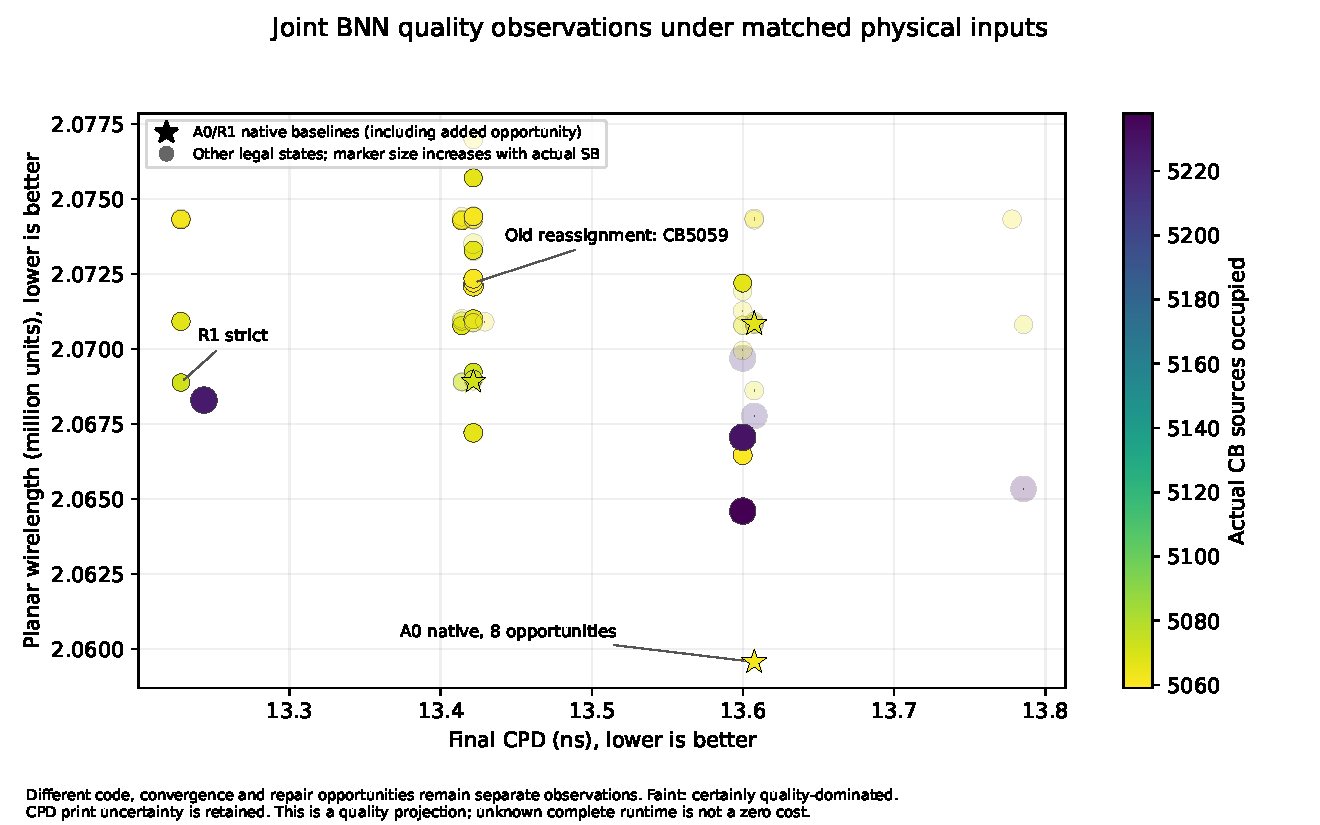
\includegraphics[width=.95\textwidth]{data/joint_quality_tradeoffs_v14.pdf}
\caption{All118 matched BNN observations in archive28 collapsed into68 distinct scalar quality groups. Strong A0/R1 and the extra-opportunity A0 control are included, alongside historical and repaired candidates. Marker size increases with actual SB occupation and color shows CB occupation; these are not silicon-area or power estimates. Faint points are certainly quality-dominated. CPD print uncertainty is retained, and quality dominance is not full-runtime dominance. The later extra-opportunity R1/Tf runs in archive30 restore already plotted quality states. Different versions, convergence conditions and repair opportunities are not a single algorithm point.}
\end{figure*}
